\documentclass[../analisi_dei_requisiti.tex]{subfiles}

\begin{document}%
\subsection{Attori}%
\label{subs:attori}

\subsubsection{Attori primari}%
\label{sssec:attori_primari}
\begin{description}
 \item \textbf{Utente}: Si fa riferimento all'utente che ha intenzione di effettuare l'analisi di un determinato dataset attraverso la \emph{exploratory data analysis (EDA)}.
\end{description}

\subsubsection{Attori secondari}
\label{sssec:attori_secondari}
\begin{description}
    \item \textbf{Database}: Fonte esterna dalla l'utente può effettuare query che ritorneranno i dati da visualizzare nei grafici.
\end{description}

\begin{figure}[h]
    \centering
    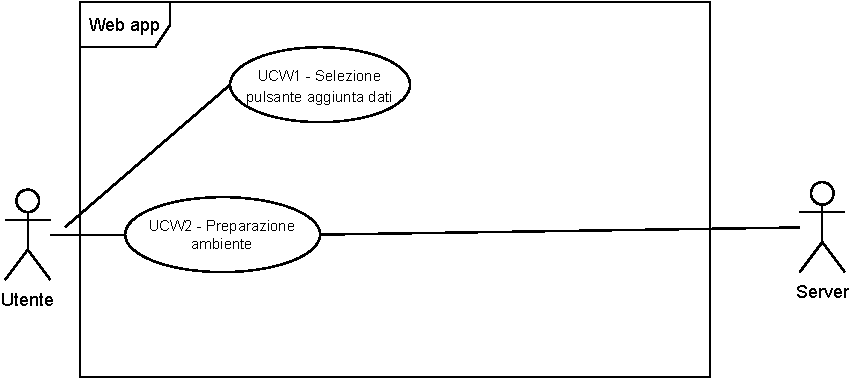
\includegraphics[width=0.7\textwidth]{diagrammi/UC0.pdf}
    \caption{Diagramma rappresentante UCW1 e UCW2}
    \label{fig:UCW0}
\end{figure}

\subsection{UCW1 - Selezione opzione aggiunta dati}
\label{sub:ucw1}

\begin{itemize}
    \item \textbf{Descrizione}: L'utente prepara seleziona l'opzione di aggiunta dei dati.
	
    \item \textbf{Attore primario}: Utente;
        
    \item \textbf{Precondizione}:   L'applicazione è in esecuzione;

	\item \textbf{Postcondizione}:  Viene selezionata l'opzione di aggiunta dei dati;

	\item \textbf{Scenario principale}:
		\begin{enumerate}
			\item L'utente seleziona l'opzione di aggiunta dei dati;
        \end{enumerate}
   
\end{itemize}

\subsection{UCW2 - Preparazione ambiente}
\label{sub:ucw2}

\begin{itemize}
    \item \textbf{Descrizione}: L'utente prepara l'applicativo HD Viz alla visualizzazione dei dati selezionando la fonte del suo dataset.
	
    \item \textbf{Attore primario}: Utente;
        
    \item \textbf{Precondizione}:   L'utente ha selezionato l'opzione di aggiunta dei dati (\hyperref[sub:ucw1]{UCW1});

    \item \textbf{Postcondizione}:  Viene selezionata la fonte dei dati desiderata;

	\item \textbf{Scenario principale}:
		\begin{enumerate}
			\item L'utente seleziona l'opzione di aggiunta dei dati;
            \item L'utente seleziona la fonte dei dati da importare;
        \end{enumerate}
   
\end{itemize}

\begin{figure}[h]
    \centering
    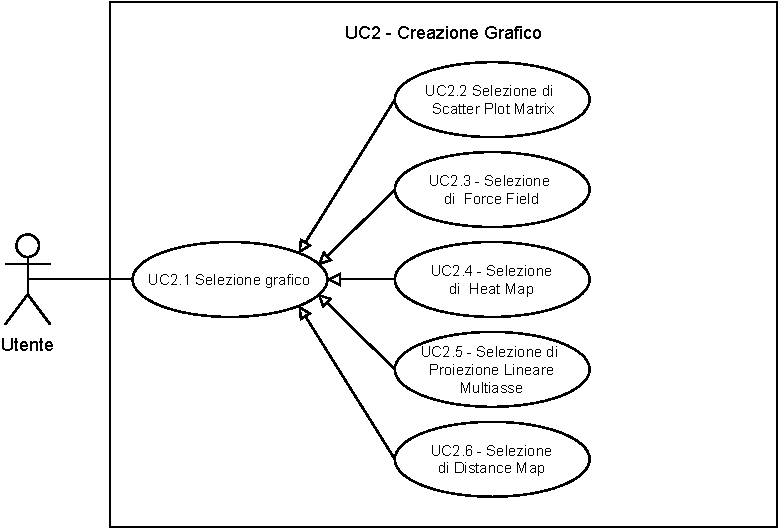
\includegraphics[width=0.7\textwidth]{diagrammi/UC2.pdf}
    \caption{Diagramma rappresentante UCW2}
    \label{fig:UCW2}
\end{figure}

\subsubsection{UCW2.1 - Selezione fonte}
\label{ssub:ucw2.1}
\begin{itemize}
    \item \textbf{Descrizione}: L'utente decide di impostare l'ambiente scegliendo la fonte di un dataset;

    \item \textbf{Attore primario}: Utente;
        
    \item \textbf{Precondizione}:   L'applicazione è in esecuzione;

    \item \textbf{Postcondizione}:  Viene selezionata la fonte del dataset;

	\item \textbf{Scenario principale}:
		\begin{enumerate}
			\item L'utente seleziona l'opzione di aggiunta dei dati:
        \end{enumerate}

        \item \textbf{Generalizzazioni}:
        \begin{enumerate}
            \item Selezione dell'opzione file csv (\hyperref[ssub:ucw2.2]{UCW2.2});
            \item Selezione dell'opzione database (\hyperref[ssub:ucw2.3]{UCW2.3}).
        \end{enumerate}
\end{itemize}


\subsubsection{UCW2.2 - Selezione del file csv}
\label{ssub:ucw2.2}
\begin{itemize}
    \item \textbf{Descrizione}: L'utente seleziona un file csv del suo dispositivo;

    \item \textbf{Attore primario}: Utente;
    
    \item \textbf{Precondizione}:   L'applicazione è in esecuzione;
    \item \textbf{Postcondizione}:  Viene selezionato un file csv;

	\item \textbf{Scenario principale}:
		\begin{enumerate}
			\item L'utente seleziona l'opzione di aggiunta dei dati mediante file;
			\item L'utente seleziona il file csv di dati da importare.
        \end{enumerate}
\end{itemize}

\subsubsection{UCW2.3 - Selezione del database}
\label{ssub:ucw2.3}
\begin{itemize}
    \item \textbf{Descrizione}: L'utente seleziona l'input da database e un file di configurazione;
	
    \item \textbf{Attore primario}: Utente;
    
    \item \textbf{Precondizione}:   L'utente decide di caricare i dati mediante un database;
    \item \textbf{Postcondizione}:  Viene selezionato l'input da database e la configurazione desiderata;

	\item \textbf{Scenario principale}:
		\begin{enumerate}
			\item L'utente seleziona l'input da database;
			\item L'utente seleziona una delle impostazioni di configurazione predefiniti.
        \end{enumerate}

\end{itemize}

\newpage
\subsection{UCW2 - Creazione grafico}
\label{sub:ucw2}

\begin{figure}[h]
    \centering
    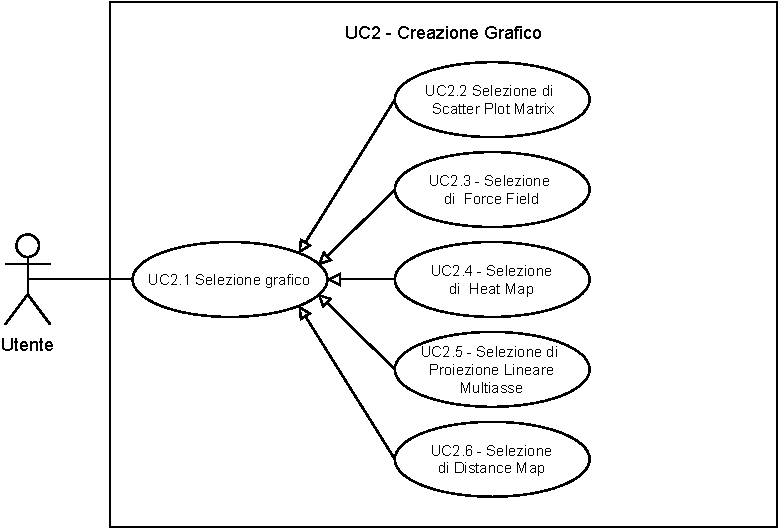
\includegraphics[width=0.8\textwidth]{diagrammi/UC2.pdf}
    \caption{Diagramma rappresentante UCW2}
    \label{fig:UCW2}
\end{figure}


\begin{itemize}
	\item \textbf{Descrizione}: L’utente seleziona dal menù di creazione di un grafico una tipologia di 
	visualizzazione, viene poi computato il relativo grafico mediante i dati caricati e infine visualizzato;
	
    \item \textbf{Attore primario}: Utente;
    
    \item \textbf{Precondizione}: É stato creato un ambiente valido (\hyperref[sub:ucs1]{UCS1});

	\item \textbf{Postcondizione}:  Viene visualizzato il grafico della tipologia scelta dall'utente a partire dai dati 
	correntemente presenti nell'ambiente; 

	\item \textbf{Scenario principale}:
		\begin{enumerate}
			\item L'utente seleziona l'opzione che desidera tra le tipologie di grafico (\hyperref[ssub:ucw2.1]{UCW2.1});
			\item Il sistema calcola il grafico della tipologia selezionata sui dati precedentemente caricati;
			\item Il sistema visualizza il grafico computato.
		\end{enumerate}
\end{itemize}

\subsubsection{UCW2.1 - Selezione grafico}
\label{ssub:ucW2.1}
\begin{itemize}

	\item \textbf{Descrizione}: L’utente seleziona la tipologia di grafico che desidera costruire;

    \item \textbf{Attore primario}: Utente;

	\item \textbf{Precondizione}:   É stato creato un ambiente valido (\hyperref[sub:ucs1]{UCS1});
	
    \item \textbf{Postcondizione}:  É stata selezionata la tipologia del grafico che verrà costruito;

	\item \textbf{Generalizzazioni}:
		\begin{enumerate}
			
			\item Selezione di Scatterplot matrix \hyperref[ssub:ucw2.2]{UCW2.2};
			\item Selezione di Force Field \hyperref[ssub:ucw2.3]{UCW2.3};
			\item Selezione di Heat Map \hyperref[ssub:ucw2.4]{UCW2.4};
			\item Selezione di Proiezione Lineare Multiasse \hyperref[ssub:ucw2.5]{UCW2.5};
			\item Selezione di Distance Map \hyperref[ssub:ucw2.6]{UCW2.6}.
			
		\end{enumerate}

\end{itemize}


\subsubsection{UCW2.2 - Selezione di Scatter Plot Matrix}
\label{ssub:ucw2.2}
\begin{itemize}

	\item \textbf{Descrizione}: L’utente seleziona \emph{Scatter Plot Matrix} come tipologia di grafico che desidera 
	costruire;

    \item \textbf{Attore primario}: Utente;

	\item \textbf{Precondizione}:   É stato creato un ambiente valido (\hyperref[sub:ucs1]{UCS1});

	\item \textbf{Postcondizione}:  L'utente ha selezionato \emph{Scatter Plot Matrix} come tipologia del grafico da 
	costruire;

	\item \textbf{Scenario Principale}:
	\begin{enumerate}
		\item L'utente seleziona \emph{Scatter Plot Matrix} come tipologia di grafico da costruire.
	\end{enumerate}
\end{itemize}


\subsubsection{UCW2.3 - Selezione di Force Field}
\label{ssub:ucw2.3}
\begin{itemize}

	\item \textbf{Descrizione}: L’utente seleziona \emph{Force Field} come tipologia di grafico che desidera 
	costruire;

    \item \textbf{Attore primario}: Utente;

    \item \textbf{Precondizione}:   É stato creato un ambiente valido (\hyperref[sub:ucs1]{UCS1});

    \item \textbf{Postcondizione}:  L'utente ha selezionato \emph{Force Field} come tipologia del grafico da 
	costruire;
	
	\item \textbf{Scenario Principale}: 
	\begin{enumerate}
		\item L'utente seleziona \emph{Force Field} come tipologia del grafico da costruire.
	\end{enumerate}

\end{itemize}


\subsubsection{UCW2.4 - Selezione di Heat Map}
\label{ssub:ucw2.4}
\begin{itemize}

	\item \textbf{Descrizione}: L’utente seleziona \emph{Heat Map} come tipologia di grafico che desidera 
	costruire;

    \item \textbf{Attore primario}: Utente;

	\item \textbf{Precondizione}:   É stato creato un ambiente valido (\hyperref[sub:ucs1]{UCS1});

    \item \textbf{Postcondizione}:  L'utente ha selezionato \emph{Heat Map} come tipologia del grafico da 
	costruire;

	\item \textbf{Scenario Principale}: 
	\begin{enumerate}
		\item L'utente seleziona \emph{Heat Map} come tipologia del grafico da costruire.
	\end{enumerate}

\end{itemize}


\subsubsection{UCW2.5 - Selezione di Proiezione Lineare Multi Asse}
\label{ssub:ucw2.5}
\begin{itemize}

	\item \textbf{Descrizione}: L’utente seleziona \emph{Proiezione Lineare Multi Asse} come tipologia di grafico che 
	desidera costruire;

    \item \textbf{Attore primario}: Utente;

    \item \textbf{Precondizione}:   É stato creato un ambiente valido (\hyperref[sub:ucs1]{UCS1});

	\item \textbf{Postcondizione}:  L'utente ha selezionato \emph{Proiezione Lineare Multi Asse} come tipologia del 
	grafico da costruire;
	
	\item \textbf{Scenario Principale}: 
	\begin{enumerate}
		\item L'utente seleziona \emph{Proiezione Lineare Multi Asse} come tipologia del grafico da costruire.
	\end{enumerate}
\end{itemize}

\subsubsection{UCW2.6 - Selezione di Distance Map}
\label{ssub:ucw2.6}
\begin{itemize}
	\item \textbf{Descrizione}: L’utente seleziona \emph{Distance Map} come tipologia di grafico che desidera 
	costruire;
	\item \textbf{Attore primario}:	Utente;
	\item \textbf{Precondizione}:	É stato creato un ambiente valido (\hyperref[sub:ucs1]{UCS1});

    \item \textbf{Postcondizione}:  L'utente ha selezionato \emph{Distance Map} come tipologia del grafico da 
	costruire;

	\item \textbf{Scenario Principale}: 
	\begin{enumerate}
		\item L'utente seleziona \emph{Distance Map} come tipologia del grafico da costruire.
	\end{enumerate}
\end{itemize}

\newpage
\subsection{UCW4 - Modifica dei Metadati}
\label{sub:ucw4}

\begin{figure}[h]
    \centering
    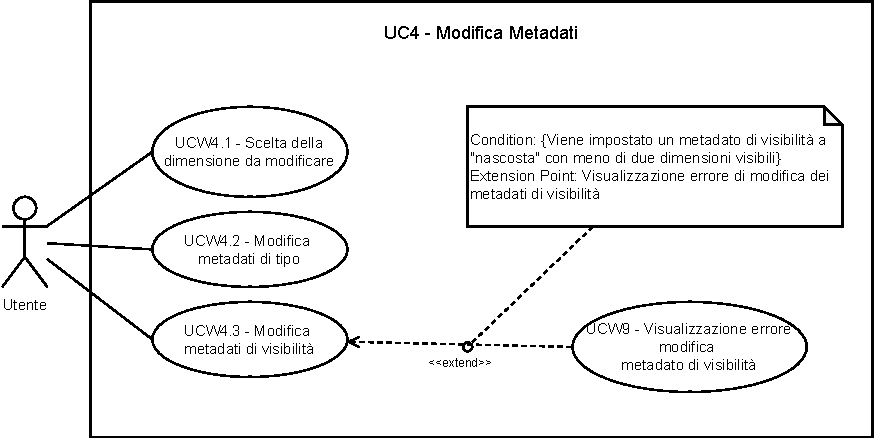
\includegraphics[width=0.7\textwidth]{diagrammi/UC4.pdf}
    \caption{Diagramma rappresentante UCW4}
    \label{fig:UCW4}
\end{figure}

%TODO: Modifica immagine
\begin{itemize}
    \item \textbf{Descrizione}: L’utente seleziona una dimensione e modifica i metadati di interesse;

    \item \textbf{Attore primario}: Utente;

    \item \textbf{Precondizione}:   É stato creato un ambiente valido (\hyperref[sub:ucs1]{UCS1});
    \item \textbf{Postcondizione}:  Sono stati aggiornati i metadati modificati della dimensione scelta dall'utente e
          sono state aggiornate eventuali visualizzazioni presenti, in accordo con i metadati aggiornati;

    \item \textbf{Scenario principale}:
          \begin{enumerate}
              \item L'utente seleziona una dimensione da modificare (\hyperref[ssub:ucw4.1]{UCW4.1});
              \item L'utente modifica il metadato di tipo e/o quello di visibilità della dimensione selezionata
                    (\hyperref[ssub:ucw4.2]{UCW4.2} e \hyperref[ssub:ucw4.3]{UCW4.3});
              \item Vengono aggiornati i metadati modificati della dimensione selezionata;
              \item Vengono aggiornate le eventuali visualizzazioni presenti, in accordo con i metadati
                    aggiornati.
          \end{enumerate}

    \item \textbf{Scenari alternativi}:
          \begin{itemize}
              \item L'utente interrompe le modifiche che stava apportando:
                    \begin{enumerate}
                        \item L'utente seleziona una dimensione da modificare (\hyperref[ssub:ucw4.1]{UCW4.1});
                        \item L'utente deseleziona la dimensione selezionata.
                    \end{enumerate}
          \end{itemize}
\end{itemize}

\newpage

\subsubsection{UCW4.1 - Scelta della dimensione da modificare}
\label{ssub:ucw4.1}

\begin{itemize}
    \item \textbf{Descrizione}: L’utente seleziona una dimensione della quale modificare i metadati;
    \item \textbf{Attore primario}: Utente;

    \item \textbf{Precondizione}:   L'utente ha aperto il menu di modifica dei metadati;
    \item \textbf{Postcondizione}:  Viene selezionata la dimensione del dataset della quale desidera modificare i
          metadati;

    \item \textbf{Scenario principale}:
          \begin{enumerate}
              \item L'utente seleziona una dimensione tra quelle del dataset corrente.
          \end{enumerate}
\end{itemize}

\subsubsection{UCW4.2 - Modifica metadato di tipo}
\label{ssub:ucw4.2}

\begin{itemize}
    \item \textbf{Descrizione}: L’utente modifica il metadato di tipo, della dimensione del dataset selezionata,
          scegliendo il nuovo valore tra le opzioni presentate;

    \item \textbf{Attore primario}: Utente;

    \item \textbf{Precondizione}:   L'utente ha selezionato una dimensione del dataset della quale desidera modificare
          i metadati (\hyperref[ssub:ucw4.1]{UCW4.1});
    \item \textbf{Postcondizione}:  Viene modificato il metadato di tipo della dimensione selezionata;

    \item \textbf{Scenario principale}:
          \begin{enumerate}
              \item L'utente seleziona il metadato di tipo della dimensione precedentemente selezionata;
              \item L'utente seleziona il valore che desidera assegnare al metadato di tipo della dimensione selezionata
                    scegliendo tra i valori proposti.
          \end{enumerate}


\end{itemize}


\subsubsection{UCW4.3 - Modifica metadato di visibilità}
\label{ssub:ucw4.3}

\begin{itemize}
    \item \textbf{Descrizione}: L’utente modifica il metadato di visibilità della dimensione del dataset selezionata;

    \item \textbf{Attore primario}: Utente;

    \item \textbf{Precondizione}:   L'utente ha selezionato una dimensione del dataset della quale desidera modificare
          i metadati (\hyperref[ssub:ucw4.1]{UCW4.1});

    \item \textbf{Postcondizione}:  Viene modificato il metadato di visibilità della dimensione selezionata;

    \item \textbf{Scenario principale}:
          \begin{enumerate}
              \item L'utente seleziona il metadato di visibilità della dimensione precedentemente selezionata;
              \item L'utente seleziona il valore che desidera assegnare al metadato di visibilità della dimensione
                    selezionata scegliendo tra i valori proposti ("visibile" e "nascosta");
          \end{enumerate}

    \item \textbf{Estensioni}:
          \begin{itemize}
              \item L'utente imposta come "nascosta" un metadato di visibilità, con meno di due dimensioni visibili:
                    \begin{enumerate}
                        \item Il metadato di visibilità della dimensione selezionata viene impostato a
                              visibile;
                        \item Viene visualizzato il messaggio di errore (\hyperref[sub:ucw9]{UCW9}).
                    \end{enumerate}
          \end{itemize}
\end{itemize}
\newpage
\subsection{UCW5 - Modifica visualizzazione}
\label{sub:ucw5}

\begin{figure}[h]
    \centering
    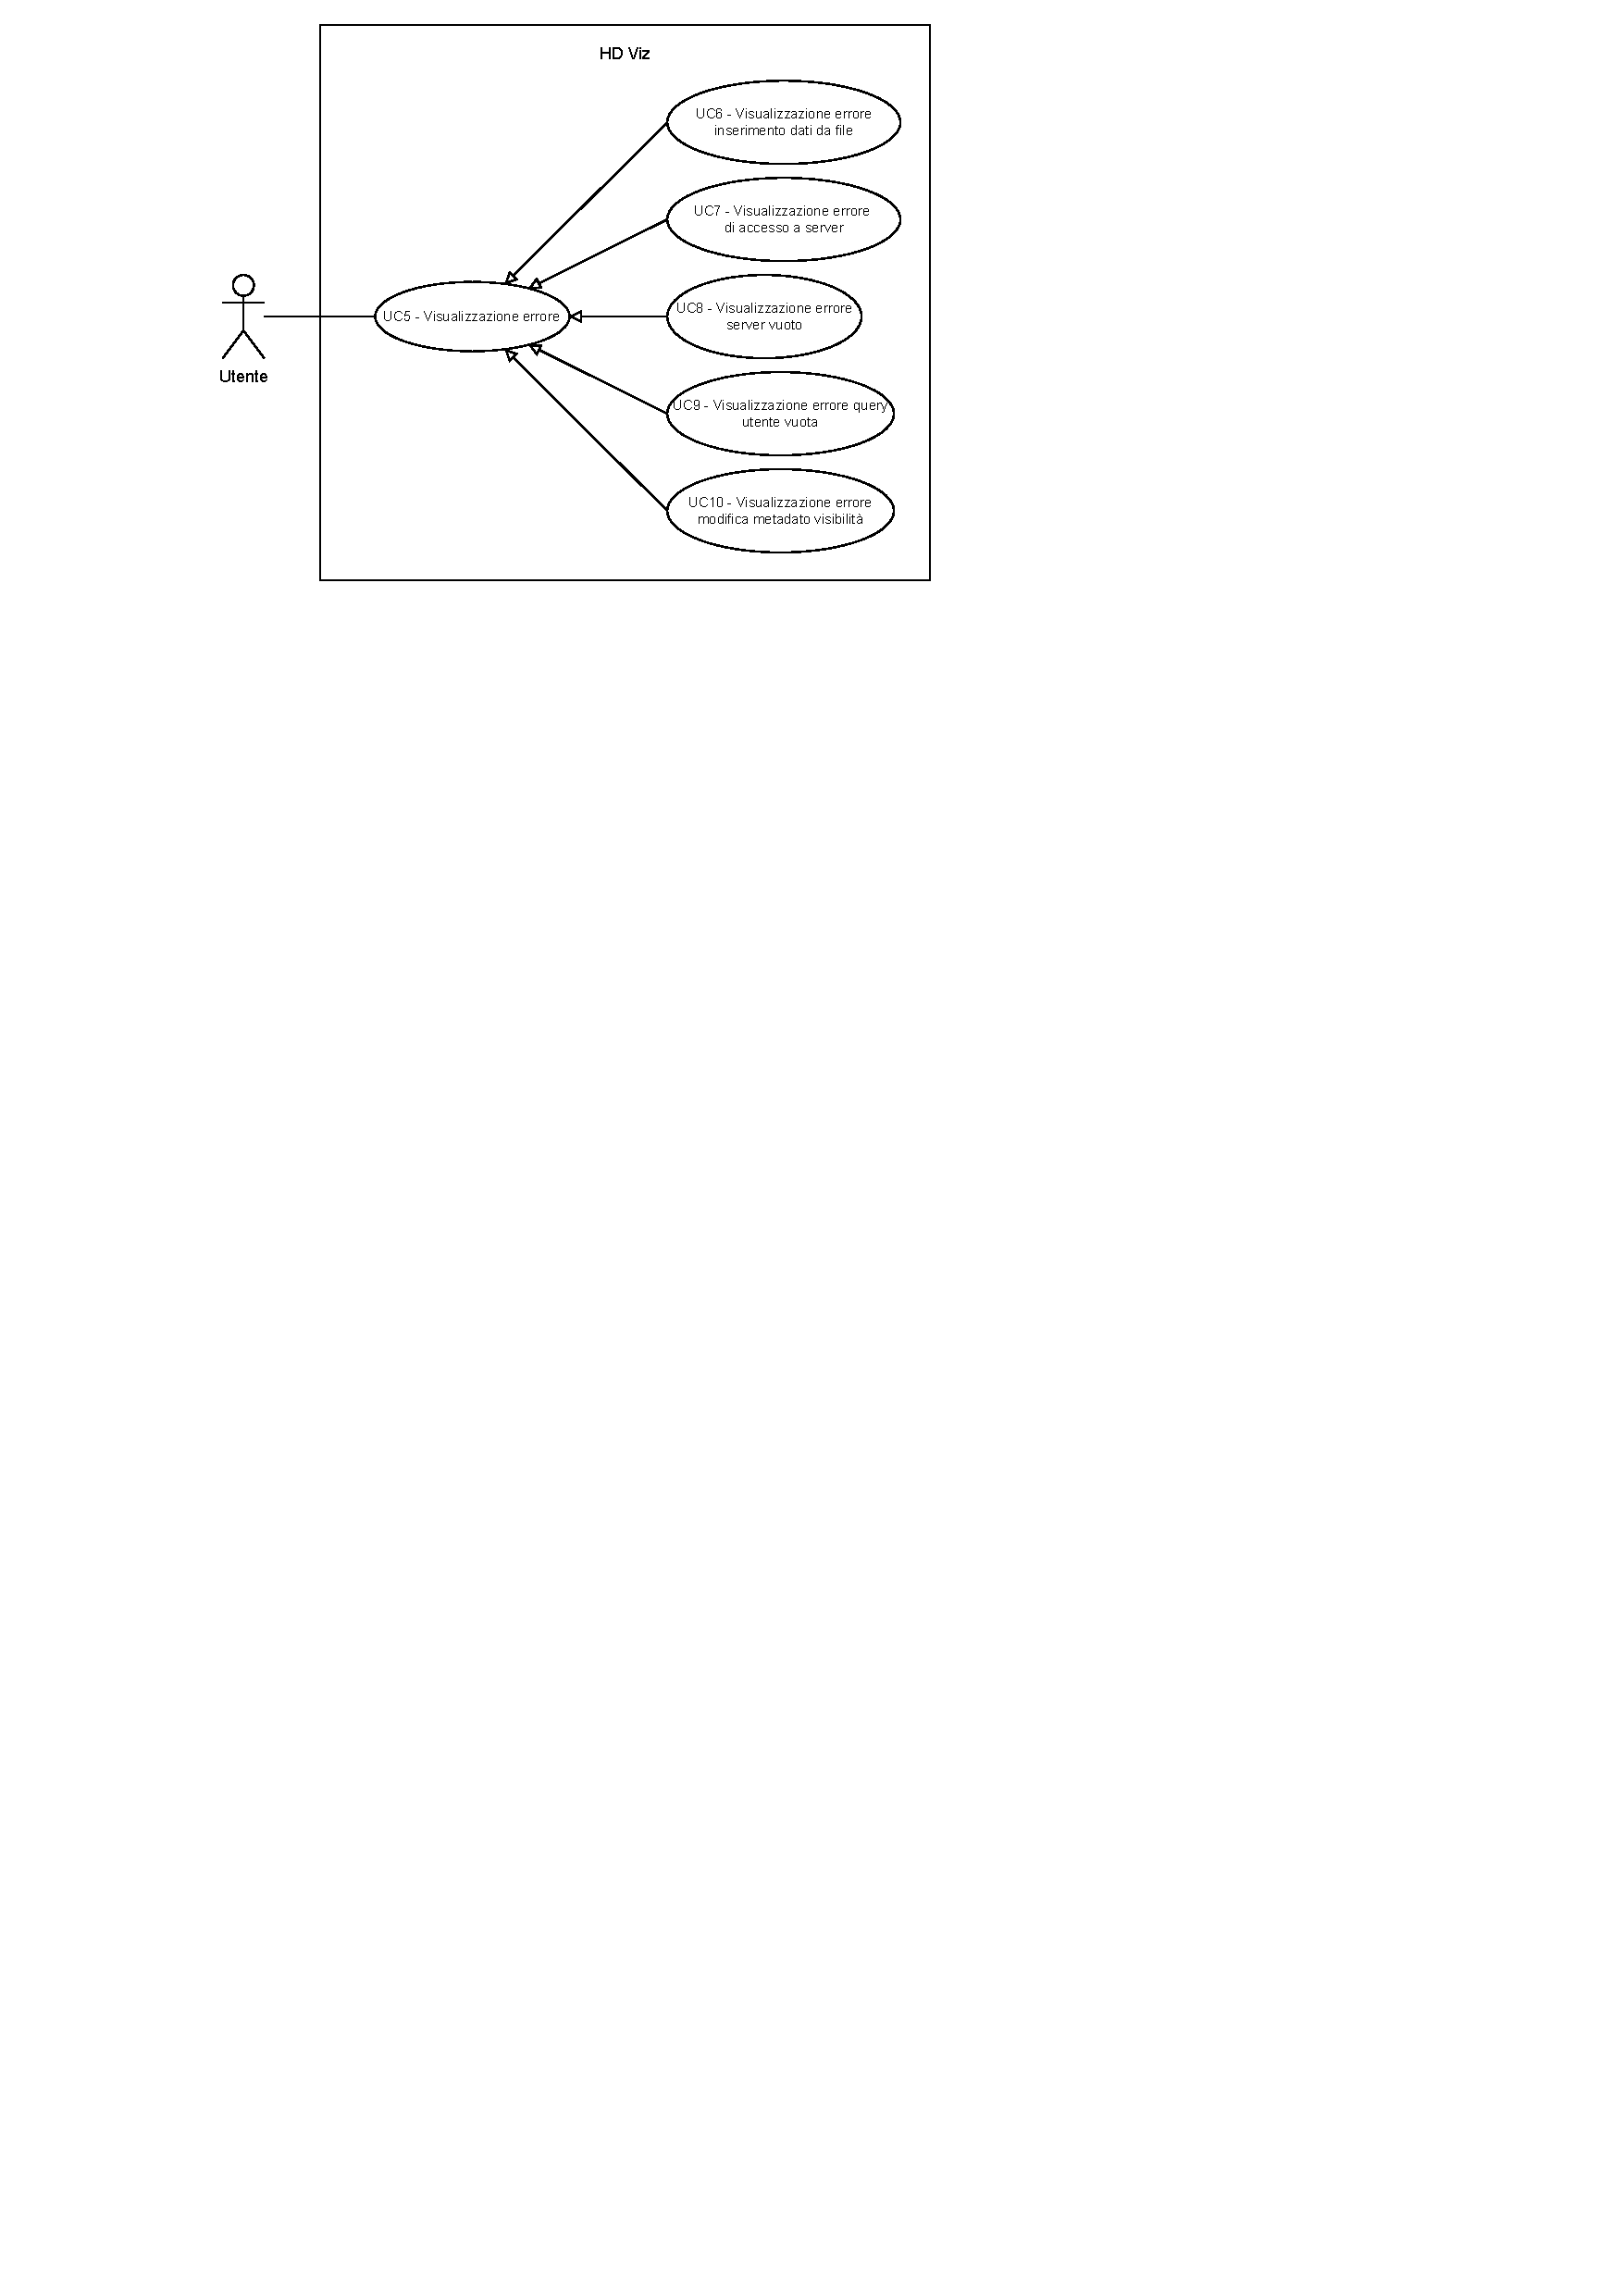
\includegraphics[width=0.8\textwidth]{diagrammi/UC5.pdf}
    \caption{Diagramma rappresentante UCW5}
    \label{fig:UCW5}
\end{figure}


\begin{itemize}
    \item \textbf{Descrizione}: L’utente modifica il grafico attuale del quale viene fornita la visualizzazione
          aggiornata;

    \item \textbf{Attore primario}: Utente;

    \item \textbf{Precondizione}:   È stato costruito correttamente un grafico (\hyperref[sub:ucw3]{UCW3});

    \item \textbf{Postcondizione}:  Viene visualizzato il grafico modificato con i nuovi parametri;

    \item \textbf{Scenario principale}:
          \begin{enumerate}
              \item L'utente modifica i parametri di visualizzazione, interagendo con gli strumenti resi disponibili dal
                    grafico che sta visualizzando, dal menu di modifica;
              \item La visualizzazione del grafico viene aggiornata in accordo con i parametri modificati.
          \end{enumerate}

    \item \textbf{Scenari alternativi}:
          \begin{itemize}
              \item Annullamento delle modifiche:
                    \begin{enumerate}
                        \item L'utente seleziona la voce "Annulla" dal menù di modifica;
                        \item Le modifiche vengono scartate e viene ripristinata la visualizzazione del grafico precedente
                              (\hyperref[ssub:ucw5.8]{UCW5.8}).
                    \end{enumerate}
          \end{itemize}

\end{itemize}

\newpage
\subsubsection{UCW5.1 - Modifica grafico}
\label{ssub:ucw5.1}

\begin{itemize}
    \item \textbf{Descrizione}: L’utente effettua modifica specifiche al tipo di grafico precedentemente costruito e visualizzato,
          su parametri quindi validi solo per tale visualizzazione, e ne vede le modifiche;

    \item \textbf{Attore primario}: Utente;

    \item \textbf{Precondizione}:   È stato costruito correttamente un grafico (\hyperref[sub:ucw3]{UCW3});

    \item \textbf{Postcondizione}:  Viene aggiornato il grafico costruito e visualizzato con i nuovi parametri;

    \item \textbf{Generalizzazioni}:
          \begin{itemize}
              \item Modifica Scatter Plot Matrix (\hyperref[ssub:ucw5.2]{UCW5.2});
              \item Modifica a grafico con Matrice delle Distanze (\hyperref[ssub:ucw5.3]{UCW5.3});
                    \begin{itemize}
                        \item Modifica Force Field (\hyperref[ssub:ucw5.4]{UCW5.4});
                        \item Modifica Distance Map (\hyperref[ssub:ucw5.5]{UCW5.5});
                    \end{itemize}
              \item Modifica Heat Map (\hyperref[ssub:ucw5.6]{UCW5.6});
              \item Modifica Proiezione Lineare Multi Asse (\hyperref[ssub:ucw5.7]{UCW5.7}).
          \end{itemize}
\end{itemize}

\subsubsection{UCW5.2 - Modifica Scatter Plot Matrix}
\label{ssub:ucw5.2}

\begin{figure}[h]
    \centering
    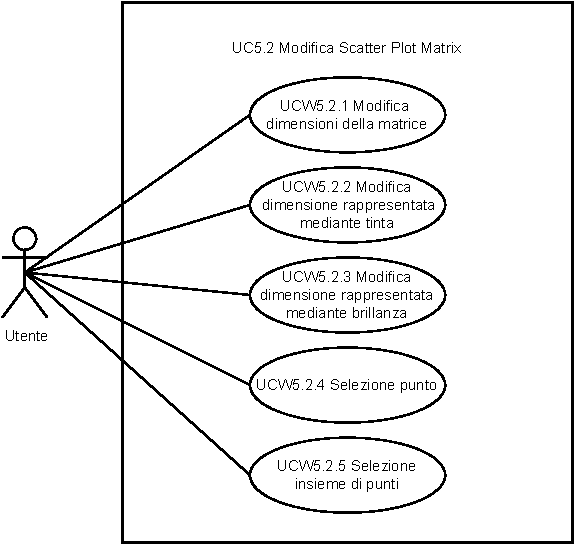
\includegraphics[width=0.6\textwidth]{diagrammi/UC5_2.pdf}
    \caption{Diagramma rappresentante UCW5.2}
    \label{fig:UCW5.2}
\end{figure}


\begin{itemize}
    \item \textbf{Descrizione}: L’utente modifica la visualizzazione dello Scatter Plot Matrix
          costruito dal dataset corrente;

    \item \textbf{Attore primario}: Utente;

    \item \textbf{Precondizione}:   La visualizzazione costruita dal dataset corrente è uno Scatter Plot Matrix;

    \item \textbf{Postcondizione}:  Viene aggiornato il grafico costruito e visualizzato con i nuovi parametri;

    \item \textbf{Scenario principale}:
          \begin{enumerate}
              \item L'utente apporta le modifiche desiderate tra quelle offerte dallo Scatter Plot Matrix.
          \end{enumerate}
\end{itemize}


\paragraph{UCW5.2.1 - Modifica dimensioni della matrice}
\label{par:ucw5.2.1}
\begin{itemize}
    \item \textbf{Descrizione}:     L’utente dispone di dati con metadati assegnati e può
          scegliere fino a 5 dimensioni che possono essere visualizzate nello Scatter Plot
          Matrix;

    \item \textbf{Attore primario}: Utente;

    \item \textbf{Precondizione}:   La visualizzazione costruita dal dataset corrente è uno Scatter Plot Matrix;
    \item \textbf{Postcondizione}:  Vengono modificate le dimensioni visualizzate nei plot dello Scatter Plot Matrix;

    \item \textbf{Scenario principale}:
          \begin{enumerate}
              \item   L'utente seleziona l'opzione di selezione delle dimensioni;
              \item   L'utente seleziona fino a cinque dimensioni;

              \item   Ad ogni selezione l'utente
                    sceglie una delle dimensioni attuali del grafico e la scarta;

              \item   La visualizzazione sostituisce le dimensioni scartate con le nuove selezionate.
          \end{enumerate}
\end{itemize}

\paragraph{UCW5.2.2 - Modifica dimensione rappresentata mediante tinta}
\label{par:ucw5.2.2}
\begin{itemize}

    \item \textbf{Descrizione}:     L'utente assegna ad una dimensione un insieme di tinte per poterla rappresentare
          graficamente;

    \item \textbf{Attore primario}: Utente;
    \item \textbf{Precondizione}:   La visualizzazione correntemente costruita dal dataset è uno Scatter Plot Matrix;
    \item \textbf{Postcondizione}:  Viene aggiunta una dimensione rappresentata mediante tinta;
    \item \textbf{Scenario principale}:
          \begin{enumerate}

              \item   Interagendo con l'apposito pulsante, l'utente seleziona la dimensione che desidera rappresentare
                    mediante tinta, sostituendo così quella precedente;

              \item   L'utente seleziona tra gli intervalli di tinte suggeriti quello con cui i diversi elementi della
                    dimensione scelta saranno visualizzati;

              \item   La visualizzazione viene aggiornata in accordo con le modifiche effettuate.
          \end{enumerate}
\end{itemize}

\paragraph{UCW5.2.3 - Modifica dimensione rappresentata mediante brillanza}
\label{par:ucw5.2.3}
\begin{itemize}

    \item \textbf{Descrizione}:     L'utente assegna ad una dimensione la rappresentazione mediante brillanza;
    \item \textbf{Attore primario}: Utente;
    \item \textbf{Precondizione}:   La visualizzazione correntemente costruita dal dataset è uno Scatter Plot Matrix;
    \item \textbf{Postcondizione}:  Viene modificata la dimensione rappresentata mediante brillanza;
    \item \textbf{Scenario principale}:
          \begin{enumerate}
              \item   Interagendo con l'apposito pulsante, l'utente seleziona la dimensione che desidera rappresentare
                    mediante brillanza, sostituendo così quella precedente;

              \item   La visualizzazione viene aggiornata in accordo con la modifica effettuata.
          \end{enumerate}
\end{itemize}

\paragraph{UCW5.2.4 - Selezione punto}
\label{par:ucw5.2.4}
\begin{itemize}
    \item \textbf{Descrizione}: L'utente seleziona un punto in uno Scatter Plot della matrice per vedere come
          esso viene rappresentato negli altri grafici a dispersione della visualizzazione corrente;

    \item \textbf{Attore primario}: Utente;

    \item \textbf{Precondizione}:   La visualizzazione costruita dal dataset corrente è uno Scatter Plot Matrix;
    \item \textbf{Postcondizione}:  Le proiezioni del punto selezionato, se appartiene al dataset importato,
          vengono evidenziate in tutti i grafici della visualizzazione;

    \item \textbf{Scenario principale}:
          \begin{enumerate}
              \item L'utente seleziona un punto contente dati di uno Scatter Plot della matrice;
              \item La proiezione del punto viene evidenziata in tutti gli Scatter Plot della visualizzazione.
          \end{enumerate}

    \item \textbf{Scenari alternativi}:
          \begin{itemize}
              \item Selezione nulla:
                    \begin{enumerate}
                        \item L'utente seleziona un punto che non rappresenta nessun dato del dataset;
                        \item Non viene evidenziato alcun punto della matrice.
                    \end{enumerate}
          \end{itemize}

\end{itemize}


\paragraph{UCW5.2.5 - Selezione insieme di punti}
\label{par:ucw5.2.5}
\begin{itemize}
    \item \textbf{Descrizione}: L'utente seleziona un insieme di punti in uno Scatter Plot della matrice per vedere come
          essi vengono rappresentati negli altri Scatterplot della matrice;

    \item \textbf{Attore primario}: Utente;

    \item \textbf{Precondizione}:   La visualizzazione costruita dal dataset corrente è uno Scatter Plot Matrix;
    \item \textbf{Postcondizione}:  Le proiezioni degli insiemi di punti selezionati, se appartenente al dataset importato,
          vengono evidenziate in tutti i grafici della visualizzazione;

    \item \textbf{Scenario principale}:
          \begin{enumerate}
              \item L'utente seleziona un insieme di punti di uno Scatter Plot della matrice;
              \item Le proiezioni dei punti contenenti dati vengono evidenziati in tutti gli Scatter Plot della visualizzazione.
          \end{enumerate}

    \item \textbf{Scenari alternativi}:
          \begin{itemize}
              \item Selezione nulla:
                    \begin{enumerate}
                        \item L'utente seleziona un insieme di punti vuoto;
                        \item Non viene evidenziato alcun punto della matrice.
                    \end{enumerate}
          \end{itemize}

\end{itemize}

\newpage
\subsubsection{UCW5.3 - Modifica a grafico con matrice delle distanze}
\label{ssub:ucw5.3}

\begin{figure}[h]
    \centering
    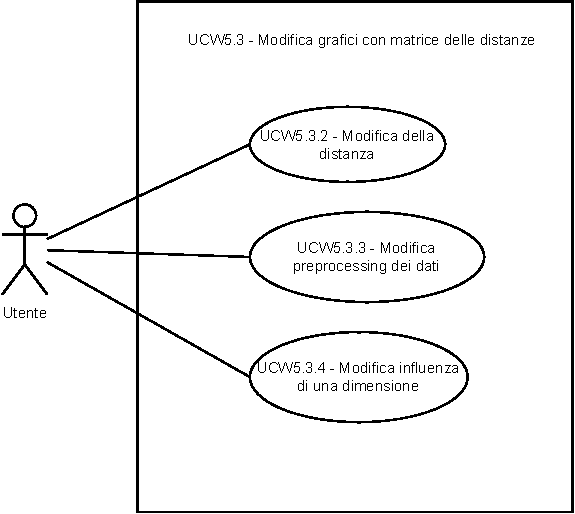
\includegraphics[width=0.8  \textwidth]{diagrammi/UC5_3.pdf}
    \caption{Diagramma rappresentante UCW5.3}
    \label{fig:UCW5.3}
\end{figure}

\begin{itemize}
    \item \textbf{Descrizione}: L’utente vuole modificare la visualizzazione di un grafico che sfrutta la matrice delle
          distanze (Force Field e Distance Map) per la sua costruzione;
    \item \textbf{Attore primario}: Utente;
    \item \textbf{Precondizione}: La visualizzazione costruita dal dataset corrente è una Force Field o una Distance Map;
    \item \textbf{Postcondizione}: Viene aggiornato e visualizzato il grafico precedentemente costruito con i parametri opportunamente modificati;
    \item \textbf{Scenario principale}:
          \begin{enumerate}
              \item L’utente apporta le modifiche desiderate tra quelle offerte dai grafici costruiti tramite matrice delle
                    distanze e quelle specifiche al tipo di grafico attualmente costruito.
          \end{enumerate}
    \item \textbf{Generalizzazioni}:
          \begin{itemize}
              \item Modifica Force Field (\hyperref[ssub:ucw5.4]{UCW5.4});
              \item Modifica Distance Map (\hyperref[ssub:ucw5.5]{UCW5.5}).
          \end{itemize}
\end{itemize}

\paragraph{UCW5.3.1 - Modifica della distanza}
\label{par:ucw5.3.1}
\begin{itemize}
    \item \textbf{Descrizione}: L’utente decide di cambiare l’algoritmo usato per il calcolo delle distanze;

    \item \textbf{Attore primario}: Utente;

    \item \textbf{Precondizione}:   L'utente ha selezionato la voce \emph{"Modifica della distanza"} da (\hyperref[ssub:uc5.3]{UC5.3});
    \item \textbf{Postcondizione}:  La visualizzazione corrente viene aggiornata in funzione della matrice delle distanze ricalcolata;

    \item \textbf{Scenario principale}:
          \begin{enumerate}
              \item L'utente seleziona uno degli algoritmi di calcolo della distanza tra "\glossario{Euclidea}",
                    "\glossario{Manhattan}", "\glossario{Minkowski}", "\glossario{Canberra}";
              \item La distanza tra i punti viene ricalcolata secondo l'algoritmo scelto;
              \item La visualizzazione del grafico precedentemente costruito viene aggiornata.
          \end{enumerate}
\end{itemize}

\paragraph{UCW5.3.2 - Modifica preprocessing dei dati}
\label{par:ucw5.3.2}
\begin{itemize}
    \item \textbf{Descrizione}: L’utente sceglie se normalizzare, standardizzare o non effettuare alcuna operazione preliminare sui dati;

    \item \textbf{Attore primario}: Utente;
    \item \textbf{Precondizione}: L'utente ha selezionato la voce \emph{"Modifica preprocessing dei dati"} da (\hyperref[ssub:ucw5.3]{UCW5.3});
    \item \textbf{Postcondizione}: La visualizzazione corrente viene aggiornata in funzione della matrice delle distanze ricalcolata;
    \item \textbf{Scenario principale}:
          \begin{enumerate}
              \item L'utente seleziona la casella \emph{"Normalizza"} o \emph{"Standardizza"};
              \item HD Viz ricalcola la matrice delle distanze in base all'opzione scelta;
              \item La visualizzazione del grafico precedentemente costruito viene aggiornata.
          \end{enumerate}
\end{itemize}

\paragraph{UCW5.3.3 - Modifica influenza di una dimensione}
\label{par:ucw5.3.3}
\begin{itemize}
    \item \textbf{Descrizione}: Per visualizzare correttamente relazioni tra i dati,
          l’utente decide di assegnare manualmente dei pesi alle dimensioni;

    \item \textbf{Attore primario}: Utente;
    \item \textbf{Precondizione}: L'utente ha selezionato la voce \emph{"Modifica influenza di una dimensione"} da (\hyperref[ssub:uc5.3]{UC5.3});

    \item \textbf{Postcondizione}: La visualizzazione corrente viene aggiornata in funzione della matrice delle distanze ricalcolata;
    \item \textbf{Scenario principale}:
          \begin{itemize}
              \item L’utente seleziona una dimensione del dataset importato e le assegna manualmente un peso;
              \item HD Viz ricalcola la matrice delle distanze con i nuovi pesi;
              \item La visualizzazione del grafico precedentemente costruito viene aggiornata.
          \end{itemize}
\end{itemize}

\newpage
\subsubsection{UCW5.4 - Modifica Force Field}
\label{ssub:ucw5.4}
% TODO: Create image for force field graph.
\begin{figure}[h]
    \centering
    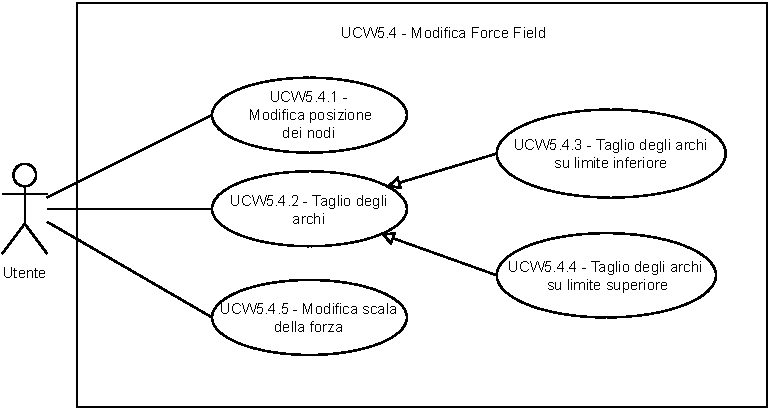
\includegraphics[width=0.6  \textwidth]{diagrammi/UC5_4.pdf}
    \caption{Diagramma rappresentante UCW5.4}
    \label{fig:UCW5.4}
\end{figure}


\begin{itemize}
    \item \textbf{Descrizione}: L’utente vuole modificare la visualizzazione del grafo Force Field
          costruito dal dataset corrente;

    \item \textbf{Attore primario}: Utente;

    \item \textbf{Precondizione}:   La visualizzazione costruita dal dataset corrente è un Force Field;

    \item \textbf{Postcondizione}:  Viene aggiornato e visualizzato il grafico precedentemente costruito con i parametri opportunamente modificati;

    \item \textbf{Scenario principale}:
          \begin{enumerate}
              \item L'utente apporta le modifiche desiderate tra quelle offerte dal Force Field.
          \end{enumerate}
\end{itemize}

\paragraph{UCW5.4.1 - Modifica posizione dei nodi}
\label{par:ucw5.4.1}
\begin{itemize}
    \item \textbf{Descrizione}: L’utente modifica la posizione dei nodi del grafo, trascinandoli nell'area definita dal grafico;

    \item \textbf{Attore primario}: Utente;

    \item \textbf{Precondizione}:   La visualizzazione costruita dal dataset corrente è un Force Field;
    \item \textbf{Postcondizione}:  Viene modificata la posizione dei nodi del grafo nella visualizzazione;

    \item \textbf{Scenario principale}:
          \begin{enumerate}
              \item L'utente clicca e trascina un nodo nello spazio della visualizzazione;
              \item La visualizzazione muove i punti del grafo mantenendo le connessioni tra i nodi.
          \end{enumerate}
\end{itemize}

\paragraph{UCW5.4.2 - Taglio degli archi}
\label{par:ucw5.4.2}
\begin{itemize}
    \item \textbf{Descrizione}:     L'utente imposta un valore di soglia sulla distanza e vengono eliminati gli archi che collegano nodi con distanza al di fuori della soglia impostata;
    \item \textbf{Attore primario}: Utente;
    \item \textbf{Precondizione}:   La visualizzazione correntemente costruita dal dataset è un Force Field;
    \item \textbf{Postcondizione}:  Viene aggiornata la visualizzazione, rimuovendo gli archi in base al valore di soglia impostato;
    \item \textbf{Scenario principale}:
          \begin{itemize}
              \item L'utente imposta una soglia;
              \item Vengono rimossi gli archi che collegano nodi che nella matrice delle distanze risultano avere una distanza che non rispetta la soglia impostata;
              \item La visualizzazione viene aggiornata con il grafo opportunamente aggiornato.
          \end{itemize}

    \item \textbf{Generalizzazioni}:
          \begin{itemize}
              \item Taglio degli archi su limite inferiore (\hyperref[par:ucw5.4.3]{UCW5.4.3});
              \item Taglio degli archi su limite superiore (\hyperref[par:ucw5.4.4]{UCW5.4.4}).
          \end{itemize}
\end{itemize}

\paragraph{UCW5.4.3 - Taglio degli archi su limite inferiore}
\label{par:ucw5.4.3}
\begin{itemize}
    \item \textbf{Descrizione}:     L'utente imposta il valore minimo della distanza e vengono eliminati gli archi che collegano nodi che nella matrice delle distanze hanno distanza minore al limite inferiore;
    \item \textbf{Attore primario}: Utente;
    \item \textbf{Precondizione}:   La visualizzazione correntemente costruita dal dataset è un Force Field;
    \item \textbf{Postcondizione}:  Viene aggiornata la visualizzazione rimuovendo gli archi  che collegano nodi tra loro distanti meno del valore di soglia minimo;
    \item \textbf{Scenario principale}:
          \begin{itemize}
              \item L'utente imposta il valore di soglia minimo;
              \item Vengono rimossi gli archi che collegano nodi che nella matrice delle distanze risultano avere una distanza inferiore alla soglia minima impostata;
              \item La visualizzazione viene aggiornata con il grafo opportunamente aggiornato.
          \end{itemize}
\end{itemize}

\paragraph{UCW5.4.4 - Taglio degli archi su limite superiore}
\label{par:ucw5.4.4}
\begin{itemize}
    \item \textbf{Descrizione}:     L'utente imposta il valore minimo della distanza e vengono eliminati gli archi che collegano nodi che nella matrice delle distanze hanno distanza maggiore al limite superiore;
    \item \textbf{Attore primario}: Utente;
    \item \textbf{Precondizione}:   La visualizzazione correntemente costruita dal dataset è un Force Field;
    \item \textbf{Postcondizione}:  Viene aggiornata la visualizzazione rimuovendo gli archi  che collegano nodi tra loro distanti più del valore di soglia massimo;
    \item \textbf{Scenario principale}:
          \begin{itemize}
              \item L'utente imposta il valore di soglia minimo;
              \item Vengono rimossi gli archi che collegano nodi che nella matrice delle distanze risultano avere una distanza superiore alla soglia massima impostata;
              \item La visualizzazione viene aggiornata con il grafo opportunamente aggiornato.
          \end{itemize}
\end{itemize}

\paragraph{UCW5.4.5 - Modifica scala della forza}
\label{par:ucw5.4.5}
\begin{itemize}
    \item \textbf{Descrizione}: L’utente decide di modificare la scala della forza di attrazione tra i nodi;


    \item \textbf{Attore primario}: Utente;

    \item \textbf{Precondizione}:   La visualizzazione correntemente costruita dal dataset è un Force Field;
    \item \textbf{Postcondizione}:  Viene modificata l'intensità della forza di attrazione tra i nodi del grafo nella visualizzazione;

    \item \textbf{Scenario principale}:
          \begin{enumerate}
              \item L'utente trascina il cursore sulla barra di intensità varia il valore dell’intensità;
              \item La visualizzazione modifica l'intensità della forza secondo il valore selezionato nel grafo;
              \item La visualizzazione viene aggiornata con il grafo opportunamente aggiornato.
          \end{enumerate}
\end{itemize}

\newpage
\subsubsection{UCW5.5 - Modifica Distance Map}
\label{ssub:ucw5.5}
% TODO: Insert image for Distance Map
\begin{figure}[h]
    \centering
    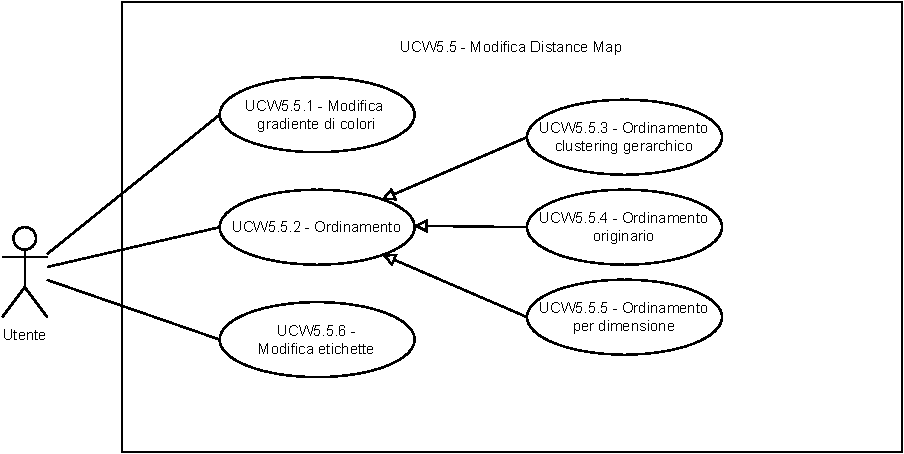
\includegraphics[width=0.8\textwidth]{diagrammi/UC5_5.pdf}
    \caption{Diagramma rappresentante UCW5.5}
    \label{fig:UCW5.5}
\end{figure}

\begin{itemize}
    \item \textbf{Descrizione}: L'utente vuole modificare la visualizzazione della Distance Map costruita dal dataset corrente;
    \item \textbf{Attore primario}: Utente;
    \item \textbf{Precondizione}: La visualizzazione costruita dal dataset corrente è un grafico di tipo Distance Map;
    \item \textbf{Postcondizione}: Viene aggiornato il grafico costruito con i nuovi parametri;
    \item \textbf{Scenario principale}:
          \begin{itemize}
              \item L'utente apporta le modifiche desiderate tra quelle offerte dalla Distance Map.
          \end{itemize}
\end{itemize}

\paragraph{UCW5.5.1 - Modifica gradiente di colori}
\label{par:ucw5.5.1}
\begin{itemize}
    \item \textbf{Descrizione}: L'utente decide di modificare la scala di colori applicata alla Distance Map scegliendo una tra le opzioni disponibili;
    \item \textbf{Attore primario}: Utente;
    \item \textbf{Precondizione}: La visualizzazione costruita dal dataset corrente è una Distance Map;
    \item \textbf{Postcondizione}: Viene modificata la scala dei colori del grafico nella visualizzazione;
    \item \textbf{Scenario principale}:
          \begin{itemize}
              \item L'utente seleziona la voce "Scala dei colori" e seleziona una tra le opzioni  "\glossario{Blue-Magenta-Yellow}", "\glossario{CoolWarm}", "\glossario{Dim Gray}";
              \item La visualizzazione cambia la scala dei colori adottata dalla Distance Map.
          \end{itemize}
\end{itemize}

\paragraph{UCW5.5.2 - Ordinamento}
\label{par:ucw5.5.2}
\begin{itemize}
    \item \textbf{Descrizione}: L'utente decide di ordinare le righe e le colonne del Distance Map al quale viene aggiunto un dendrogramma alla visualizzazione corrente;
    \item \textbf{Attore primario}: Utente;
    \item \textbf{Precondizione}: La visualizzazione costruita dal dataset corrente è una Distance Map;
    \item \textbf{Postcondizione}: Le righe e le colonne del Distance Map vengono visualizzate ordinate;
    \item \textbf{Scenario principale}:
          \begin{itemize}
              \item L'utente seleziona la casella di ordinamento;
              \item Le righe e le colonne della Distance Map vengono visualizzate secondo l'ordinamento selezionato.
          \end{itemize}
\end{itemize}

\paragraph{UCW5.5.3 - Ordinamento clustering gerarchico}
\label{par:ucw5.5.3}
\begin{itemize}
    \item \textbf{Descrizione}: L'utente decide di ordinare le righe e le colonne del Distance Map con l'algoritmo di clustering gerarchico il quale aggiunge un dendrogramma alla visualizzazione corrente;
    \item \textbf{Attore primario}: Utente;
    \item \textbf{Precondizione}: La visualizzazione costruita dal dataset corrente è una Distance Map;
    \item \textbf{Postcondizione}: Le righe e le colonne del Distance Map vengono visualizzate secondo l'ordine impostato dall'algoritmo di clustering gerarchico e con annesso il dendrogramma prodotto dall'ordinamento;
    \item \textbf{Scenario principale}:
          \begin{itemize}
              \item L'utente seleziona la casella di ordinamento delle colonne;
              \item Le righe e le colonne della Distance Map vengono visualizzate secondo l'ordinamento del clustering gerarchico e viene aggiunto il dendrogramma al grafico.
          \end{itemize}
\end{itemize}

\paragraph{UCW5.5.4 - Ordinamento originario}
\label{par:ucw5.5.4}
\begin{itemize}
    \item \textbf{Descrizione}: L'utente decide di ordinare le righe e le colonne del Distance Map seguendo l'ordine originario del dataset corrente;
    \item \textbf{Attore primario}: Utente;
    \item \textbf{Precondizione}: La visualizzazione costruita dal dataset corrente è una Distance Map;
    \item \textbf{Postcondizione}: Le righe e le colonne del Distance Map vengono visualizzate secondo l'ordine originario del dataset corrente;
    \item \textbf{Scenario principale}:
          \begin{itemize}
              \item L'utente seleziona la casella di ordinamento delle colonne;
              \item Le righe e le colonne della Distance Map vengono ordinate;
              \item Il grafico viene visualizzato aggiornato.
          \end{itemize}
\end{itemize}

\paragraph{UCW5.5.5 - Ordinamento per dimensione}
\label{par:ucw5.5.5}
\begin{itemize}
    \item \textbf{Descrizione}: L'utente decide di ordinare in maniera crescente le righe e le colonne del Distance Map secondo il valore delle dimensioni;
    \item \textbf{Attore primario}: Utente;
    \item \textbf{Precondizione}: La visualizzazione costruita dal dataset corrente è una Distance Map;
    \item \textbf{Postcondizione}: Le righe e le colonne del Distance Map vengono visualizzate ordinate secondo il valore delle dimensioni;
    \item \textbf{Scenario principale}:
          \begin{itemize}
              \item L'utente seleziona la casella di ordinamento delle colonne;
              \item Le righe e le colonne della Distance Map vengono ordinate;
              \item Il grafico viene visualizzato aggiornato.
          \end{itemize}
\end{itemize}


\paragraph{UCW5.5.6 - Modifica etichette}
\label{par:ucw5.5.6}
\begin{itemize}
    \item \textbf{Descrizione}: L'utente decide di modificare una etichetta associata alla Distance Map;
    \item \textbf{Attore primario}: Utente;
    \item \textbf{Precondizione}: La visualizzazione costruita dal dataset corrente è una Distance Map;
    \item \textbf{Postcondizione}: Le etichette della Distance Map vengono modificate secondo la scelta effettuata dall'utente;
    \item \textbf{Scenario principale}:
          \begin{itemize}
              \item L'utente sceglie una etichetta da modificare;
              \item L'utente sceglie una dimensione del dato da utilizzare come etichetta;
              \item Viene aggiornata l'etichetta nella Distance Map.
          \end{itemize}
\end{itemize}


\newpage
\subsubsection{UCW5.6 - Modifica Proiezione Lineare Multi Asse}
\label{ssub:ucw5.6}
% TODO: Create image for PLMA
\begin{figure}[h]
    \centering
    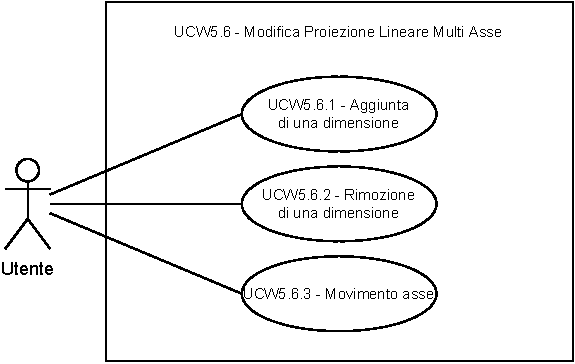
\includegraphics[width=0.8\textwidth]{diagrammi/UC5_6.pdf}
    \caption{Diagramma rappresentante UCW5.6}
    \label{fig:UCW5.6}
\end{figure}

\begin{itemize}
    \item \textbf{Descrizione}: L’utente vuole modificare la visualizzazione della Proiezione Lineare Multi Asse
          costruita dal dataset corrente;

    \item \textbf{Attore primario}: Utente;

    \item \textbf{Precondizione}:   La visualizzazione costruita dal dataset corrente è un grafico di tipo Proiezione Lineare Multi Asse;
    \item \textbf{Postcondizione}:  Viene aggiornato il grafico costruito con i nuovi parametri;

    \item \textbf{Scenario principale}:
          \begin{enumerate}
              \item L'utente apporta le modifiche desiderate tra quelle offerte dalla Proiezione Lineare Multi Asse.
          \end{enumerate}
\end{itemize}

\paragraph{UCW5.6.1 - Aggiunta dimensione}
\label{par:ucw5.6.1}
\begin{itemize}
    \item \textbf{Descrizione}: L’utente aggiunge una dimensione del dataset importato al grafico;

    \item \textbf{Attore primario}: Utente;

    \item \textbf{Precondizione}:   La visualizzazione costruita dal dataset corrente è una Proiezione Lineare Multi Asse
          e rappresenta al più una dimensione in meno rispetto al numero di dimensioni del dataset;
    \item \textbf{Postcondizione}:  Alla visualizzazione della Proiezione Lineare Multi Asse viene aggiunta una dimensione;

    \item \textbf{Scenario principale}:
          \begin{enumerate}
              \item L'utente seleziona la voce "Dimensioni" e seleziona una dimensione da aggiungere alla proiezione;
              \item La visualizzazione aggiunge la dimensione selezionata e riposiziona i punti.
          \end{enumerate}
\end{itemize}

\paragraph{UCW5.6.2 - Rimozione dimensione}
\label{par:ucw5.6.2}
\begin{itemize}
    \item \textbf{Descrizione}: L’utente decide di rimuovere una dimensione dalla Proiezione Lineare Multi Asse
          a patto che essa non sia monodimensionale;

    \item \textbf{Attore primario}: Utente;

    \item \textbf{Precondizione}:   La visualizzazione costruita dal dataset corrente è una Proiezione Lineare Multi Asse
          e rappresenta almeno due dimensioni;
    \item \textbf{Postcondizione}:  Alla visualizzazione della Proiezione Lineare Multi Asse viene rimossa una dimensione;

    \item \textbf{Scenario principale}:
          \begin{enumerate}
              \item L'utente seleziona la voce "Dimensioni" e seleziona una dimensione da rimuovere dalla proiezione;
              \item La visualizzazione rimuove la dimensione selezionata e riposiziona i punti.
          \end{enumerate}
\end{itemize}

\paragraph{UCW5.6.3 - Rotazione asse}
\label{par:ucw5.6.3}
\begin{itemize}
    \item \textbf{Descrizione}: L'utente ruota gli assi nella visualizzazione per visualizzare diverse proiezioni dello stesso dataset;
    \item \textbf{Attore primario}: Utente;
    \item \textbf{Precondizione}: La visualizzazione costruita dal dataset corrente è una Proiezione Lineare Multi Asse;
    \item \textbf{Postcondizione}: Il grafico viene ridisegnato con gli assi opportunamente ruotati;
    \item \textbf{Scenario principale}:
          \begin{enumerate}
              \item L'utente trascina un asse del grafico ruotandolo;
              \item La visualizzazione viene aggiornata con l'asse ruotandolo.
          \end{enumerate}
\end{itemize}

\newpage

\subsubsection{UCW5.7 - Modifica Heat Map}
\label{ssub:ucw5.7}
% TODO: Create image for force field graph.
\begin{figure}[h]
    \centering
    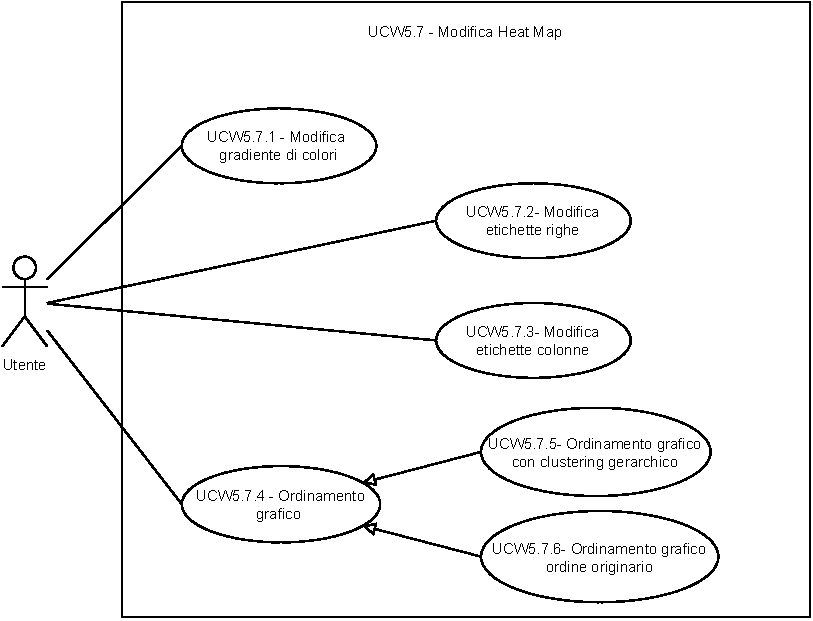
\includegraphics[width=0.6\textwidth]{diagrammi/UC5_7.pdf}
    \caption{Diagramma rappresentante UCW5.7}
    \label{fig:UCW5.7}
\end{figure}


\begin{itemize}
    \item \textbf{Descrizione}: L’utente modifica la visualizzazione della Heat Map correntemente visualizzata;

    \item \textbf{Attore primario}: Utente;

    \item \textbf{Precondizione}:   La visualizzazione correntemente costruita dal dataset è una Heat Map;

    \item \textbf{Postcondizione}:  Viene aggiornata la visualizzazione secondo i nuovi parametri impostati;

    \item \textbf{Scenario principale}:
          \begin{enumerate}
              \item L'utente apporta le modifiche desiderate tra quelle offerte dalla Heat Map.
          \end{enumerate}
\end{itemize}

\paragraph{UCW5.7.1 - Modifica gradiente di colori}
\label{par:ucw5.7.1}
\begin{itemize}
    \item \textbf{Descrizione}: L'utente decide di modificare la scala di colori applicata alla Heat Map scegliendo una tra le opzioni disponibili;

    \item \textbf{Attore primario}: Utente;

    \item \textbf{Precondizione}:   La visualizzazione costruita dal dataset corrente è una Heat Map;
    \item \textbf{Postcondizione}:  Viene modificata la scala dei colori del grafico nella visualizzazione;

    \item \textbf{Scenario principale}:
          \begin{enumerate}
              \item L'utente seleziona la voce "Scala dei colori" e seleziona una tra le opzioni  "\glossario{Blue-Magenta-Yellow}", "\glossario{CoolWarm}", "\glossario{Dim Gray}";
              \item La visualizzazione cambia la scala dei colori adottata dalla Heat Map.
          \end{enumerate}
\end{itemize}

\paragraph{UCW5.7.2 - Modifica etichette delle righe}
\label{par:ucw5.7.2}
\begin{itemize}
    \item \textbf{Descrizione}:     L'utente modifica l'etichetta associata alle righe della Heat Map;
    \item \textbf{Attore primario}: Utente;
    \item \textbf{Precondizione}:   La visualizzazione correntemente costruita dal dataset è una Heat Map;
    \item \textbf{Postcondizione}:  Le etichette delle righe dell'Heat Map vengono modificate secondo la scelta effettuata dall'utente;
    \item \textbf{Scenario principale}:
          \begin{enumerate}
              \item L'utente sceglie una etichetta da modificare;
              \item L'utente sceglie una dimensione del dato da utilizzare come etichetta;
              \item Viene aggiornata l'etichetta nella Distance Map.
          \end{enumerate}
\end{itemize}

\paragraph{UCW5.7.3 - Modifica etichette delle colonne}
\label{par:ucw5.7.3}
\begin{itemize}
    \item \textbf{Descrizione}:     L'utente modifica l'etichetta associata alla colonna della Heat Map;
    \item \textbf{Attore primario}: Utente;
    \item \textbf{Precondizione}:   La visualizzazione correntemente costruita dal dataset è una Heat Map;
    \item \textbf{Postcondizione}:  Le etichette delle colonne dell'Heat Map vengono modificate secondo la scelta effettuata dall'utente;
    \item \textbf{Scenario principale}:
          \begin{enumerate}
              \item L'utente sceglie una etichetta da modificare;
              \item L'utente sceglie una dimensione del dato da utilizzare come etichetta;
              \item Viene aggiornata l'etichetta nella Distance Map.
          \end{enumerate}
\end{itemize}

\paragraph{UCW5.7.4 - Ordinamento grafico}
\label{par:ucw5.7.4}
\begin{itemize}
    \item \textbf{Descrizione}:     L'utente modifica l'ordinamento delle colonne della visualizzazione;
    \item \textbf{Attore primario}: Utente;
    \item \textbf{Precondizione}:   La visualizzazione correntemente costruita dal dataset è una Heat Map;
    \item \textbf{Postcondizione}:  L'ordine delle colonne viene modificato;
    \item \textbf{Scenario principale}:
          \begin{enumerate}
              \item L'utente seleziona uno tra i possibili ordinamenti delle colonne;
              \item L'ordinamento del grafico viene modificato in base a quanto precedentemente selezionato;
          \end{enumerate}
    \item \textbf{Generalizzazioni}:
          \begin{itemize}
              \item Ordinamento clustering gerarchico (\hyperref[spar:ucw4.7.5]{UCW4.7.5});
              \item Ordinamento secondo ordine originario (\hyperref[spar:ucw4.7.6]{UCW4.7.6}).
          \end{itemize}
\end{itemize}

\subparagraph{UCW5.7.5 - Ordinamento grafico mediante clustering gerarchico}
\label{spar:ucw5.7.5}
\begin{itemize}
    \item \textbf{Descrizione}:     L'utente modifica l'ordinamento del grafico  della visualizzazione secondo l'algoritmo di clustering gerarchico;
    \item \textbf{Attore primario}: Utente;
    \item \textbf{Precondizione}:   La visualizzazione correntemente costruita dal dataset è una Heat Map;
    \item \textbf{Postcondizione}:  L'ordine delle colonne viene modificato in accordo con il risultato dell'applicazione dell'algoritmo di clustering gerarchico;
    \item \textbf{Scenario principale}:
          \begin{enumerate}
              \item L'utente seleziona l'ordinamento delle colonne con clustering gerarchico;
              \item L'ordinamento delle colonne della visualizzazione viene modificato in base al risultato dell'algoritmo di clustering gerarchico;
              \item Viene aggiunto sull'asse orizzontale il dendrogramma associato alla clusterizzazione.
          \end{enumerate}
\end{itemize}

\subparagraph{UCW5.7.6 - Ordinamento grafico secondo ordine originario }
\label{spar:ucw5.7.6}
\begin{itemize}
    \item \textbf{Descrizione}:     L'utente modifica l'ordinamento del grafico secondo l'ordine in cui i dati sono disposti nel dataset;
    \item \textbf{Attore primario}: Utente;
    \item \textbf{Precondizione}:   La visualizzazione correntemente costruita dal dataset è una Heat Map ed è stato selezionato il bottone "Ordina" all'interno del campo "Colonne";
    \item \textbf{Postcondizione}:  L'ordine delle colonne viene modificato in accordo con il risultato dell'applicazione dell'algoritmo di clustering gerarchico;
    \item \textbf{Scenario principale}:
          \begin{enumerate}
              \item L'utente seleziona l'ordinamento delle colonne con clustering gerarchico;
              \item L'ordinamento delle colonne della visualizzazione viene modificato in base al risultato dell'algoritmo di clustering gerarchico;
              \item Viene aggiunto sull'asse orizzontale il dendrogramma associato alla clusterizzazione.
          \end{enumerate}
\end{itemize}



\subsubsection{UCW5.8 - Annullamento delle modifiche}
\label{ssub:ucw5.8}
\begin{itemize}
    \item \textbf{Descrizione}: L'utente decide di scartare le modifiche fatte nella corrente selezione di modifica;

    \item \textbf{Attore primario}: Utente;

    \item \textbf{Precondizione}:   L'utente ha selezionato la voce di Modifica Grafico dal menù;
    \item \textbf{Postcondizione}:  Viene ripristinato il grafo ai parametri precedenti della selezione e visualizzato;

    \item \textbf{Scenario principale}:
          \begin{enumerate}
              \item L'utente seleziona il pulsante "Annulla modifiche";
              \item HD Viz ripristina i parametri del grafo ai valori precedenti alla selezione del menu di modifica.
          \end{enumerate}
\end{itemize}

\newpage
\subsection{UCW5 - Visualizzazione errore inserimento dati da file}
\label{sub:ucw5}
\begin{itemize}
    \item \textbf{Descrizione}: L'utente visualizza un messaggio di errore dopo aver caricato un file CSV non corretto 
    o vuoto;

    \item \textbf{Attore primario}: Utente;
    
    \item \textbf{Precondizione}:   L'utente carica un file CSV non corretto o vuoto (\hyperref[ssub:ucs1.2]{UCS1.2});

    \item \textbf{Postcondizione}:  Viene visualizzato un messaggio di errore relativo alla non correttezza del file 
    caricato;

    \item \textbf{Scenario principale}:
    \begin{enumerate}
        \item Viene visualizzato un messaggio d'errore relativo alla non correttezza del file caricato;
        \item L'utente conferma la presa visione dell'errore.
    \end{enumerate}

\end{itemize}

%TODO aggiungere altri casi d'uso

\end{document}